
\documentclass[12pt, twoside]{book}
%%%%%%%% Preamble %%%%%%%%%%%%
\title{Degree project}
\usepackage[utf8]{inputenc} % File coding uses utf8
\usepackage{amsmath} % Extra commands for math
\usepackage{amssymb} % Math symbols 
\usepackage{graphicx} % Include images in LaTeX
\usepackage{color} % Coloring text
\usepackage{enumerate}
\usepackage{float} % Allow you to use [H] specifier to force the position of the images 
\usepackage{capt-of} % Defines a command \captionof for putting a caption to something that’s not a float.
\usepackage{sidecap} % Defines environments called SCfigure and SCtable (analogous to figure and table) to typeset captions sideways
	\sidecaptionvpos{figure}{c} % Alignment
\usepackage{caption} % to customize the captions in floating environments like figure and table
\usepackage{commath} % Mathematics typesetting support
\usepackage{cancel} % Place lines through maths formulae
\usepackage{anysize} % to set up document margins
%\marginsize{2cm}{2cm}{2cm}{2cm} % Left, right, up, down
%\usepackage[top=2cm,bottom=4cm,left=1.5cm,right=3cm,asymmetric]{geometry}
\usepackage{appendix} %Extra control of appendices
\usepackage{tocbibind}


%EXTRA PACKAGES
\usepackage{multirow}
\usepackage{glossaries}
\usepackage[linesnumbered,ruled,vlined]{algorithm2e}
\usepackage{multirow}
\usepackage{enumerate}
\usepackage{changepage}
\usepackage{alltt}
\usepackage{listings}
\usepackage{lmodern}
\usepackage{gensymb}
\usepackage{caption}
\usepackage{subcaption}
\usepackage{hyperref}
\hypersetup{
    colorlinks,
    citecolor=blue,
    filecolor=black,
    linkcolor=black,
    urlcolor=black
}
\usepackage{listings}
\usepackage{color}
\lstloadlanguages{C,C++,csh,Java}

\definecolor{red}{rgb}{0.6,0,0} 
\definecolor{blue}{rgb}{0,0,0.6}
\definecolor{green}{rgb}{0,0.8,0}
\definecolor{cyan}{rgb}{0.0,0.6,0.6}

\lstset{
language=csh,
basicstyle=\footnotesize\ttfamily,
numbers=left,
numberstyle=\tiny,
numbersep=5pt,
tabsize=2,
extendedchars=true,
breaklines=true,
frame=b,
stringstyle=\color{blue}\ttfamily,
showspaces=false,
showtabs=false,
xleftmargin=17pt,
framexleftmargin=17pt,
framexrightmargin=5pt,
framexbottommargin=4pt,
commentstyle=\color{green},
morecomment=[l]{//}, %use comment-line-style!
morecomment=[s]{/*}{*/}, %for multiline comments
showstringspaces=false,
morekeywords={ abstract, event, new, struct,
as, explicit, null, switch,
base, extern, object, this,
bool, false, operator, throw,
break, finally, out, true,
byte, fixed, override, try,
case, float, params, typeof,
catch, for, private, uint,
char, foreach, protected, ulong,
checked, goto, public, unchecked,
class, if, readonly, unsafe,
const, implicit, ref, ushort,
continue, in, return, using,
decimal, int, sbyte, virtual,
default, interface, sealed, volatile,
delegate, internal, short, void,
do, is, sizeof, while,
double, lock, stackalloc,
else, long, static,
enum, namespace, string},
keywordstyle=\color{cyan},
identifierstyle=\color{red},
backgroundcolor=\color{white},
}

\usepackage{caption}
\DeclareCaptionFont{white}{\color{white}}
\DeclareCaptionFormat{listing}{\colorbox{blue}{\parbox{\textwidth}{\hspace{15pt}#1#2#3}}}
\captionsetup[lstlisting]{format=listing,labelfont=white,textfont=white, singlelinecheck=false, margin=0pt, font={bf,footnotesize}}

\lstdefinestyle{sharpc}{language=[Sharp]C, frame=lr, rulecolor=\color{blue!80!black}}

% Reset page margins properly for doublesided pages
\setlength{\marginparwidth}{0pt}
\setlength{\marginparsep}{0pt}
\setlength{\oddsidemargin}{0.125in}
\setlength{\evensidemargin}{0.125in}
\setlength{\textwidth}{6.375in}
\raggedbottom


%%% Theorem-like environments %%%%%%%%%%%%%%%%%%%%%%%%%%%%%%%%%%%%%%%%%%%%%%%%%%
%%\usepackage{mathtools}

\newtheorem{theorem}{Theorem}
\newtheorem{corollary}{Corollary}
\newtheorem{lemma}{Lemma}
\newtheorem{proposition}{Proposition}
\newtheorem{conjecture}{Conjecture}
\newtheorem{definition}{Definition}
\newtheorem{remark}{Remark}
\newtheorem{example}{Example}

%%%%%%%%%%%%%%%%%%%%%%%%%%%%%%%%%%%%%%%%%%%%%%%%%%%%%%%%%%%%%%%%%%%%%%%%%%%%%%%%

%%% Put your local definitions here %%%%%%%%%%%%%%%%%%%%%%%%%%%%%%%%%%%%%%%%%%%%
% For example,
\newcommand{\R}{\mathbb{R}}


% Header and Footer
\usepackage{fancyhdr} 
\pagestyle{fancy}
\fancyhf{}
\fancyhead[L]{\footnotesize University of Science and Technology of Hanoi} 
\fancyfoot[R]{\footnotesize Bachelor Thesis}  
\fancyfoot[C]{\thepage}  % center
\fancyfoot[L]{\footnotesize Information and communications technology}  %left
\renewcommand{\footrulewidth}{0.4pt}
\fancypagestyle{firststyle}
{
   \fancyhf{}
}

\usepackage{listings} % To use source code
\definecolor{dkgreen}{rgb}{0,0.6,0} % Color for using code
\definecolor{gray}{rgb}{0.5,0.5,0.5} 
% Language to use

\title{Degree project}


% \usepackage{glossaries}
\makeglossaries
\newglossaryentry{maths}
{
    name=mathematics,
    description={Mathematics is what mathematicians do}
}

\newglossaryentry{latex}
{
    name=latex,
    description={Is a mark up language specially suited for 
scientific documents}
}


\newglossaryentry{formula}
{
    name=formula,
    description={A mathematical expression}
}


%%%%%%%% Preamble ends %%%%%%%%%%%%

\begin{document}
\linespread{1.25}
%%%%%%%%%%%%%%%%%%%%%%%%%%%%%%%% Cover Page %%%%%%%%%%%%%%%%%%%%%%%%%%%%%%%%%%%%%%%%%%%

\thispagestyle{firststyle}
\begin{center}
  \begin{minipage}{0.48\textwidth} 
    \begin{center}
        
\includegraphics[scale = 0.2]{images/usth_logo.png}
    \end{center}
  \end{minipage}
  \vspace*{-3cm}

  \vspace*{1cm}

  \textsc{\Large University of Science and Technology of Hanoi}\\[1.5cm]

  \begin{minipage}{0.9\textwidth} 
    \begin{center}
      \textsc{\LARGE Bachelor Thesis}
    \end{center}
  \end{minipage}\\[0.5cm]
  
  \vspace*{1cm}

  { \huge \bfseries Hateful memes classification}\\[0.4cm]	

  \vspace*{0.5cm}
  { \large 
    \emph{Authors:} \\	
      {VU Dinh Anh} \\
      {USTHBI9-037} \\
    \vspace*{1.5cm}
    \emph{Supervisor:} \\													
      Dr. TRAN Hoang Tung, USTH ICT Lab \\
  }

  \begin{center}
    {Hanoi - July, 2021}
  \end{center}
  
\end{center}
																		
%%%%%%%%%%%%%%%%%%%% Cover page ends %%%%%%%%%%%%%%%%%%%%%%%%%%%%%%%%


\frontmatter

\chapter{Acknowledgments}
\label{chap:acknowledgments}
Yo, \textbf{[Your Name]}, con cédula de identidad \textbf{[Your ID Number]}, declaro que las ideas, juicios, valoraciones, interpretaciones, consultas bibliográficas, definiciones y conceptualizaciones expuestas en el presente trabajo; así cómo, los procedimientos y herramientas utilizadas en la investigación, son de absoluta responsabilidad de el autor del trabajo de integración curricular. Así mismo, me acojo a los reglamentos internos de la Universidad de Investigación de Tecnología Experimental Yachay. \\

\noindent Urcuquí, Marzo del 2020. \\
\ \\
\ \\

\begin{center}
    \rule[0mm]{60mm}{0.1mm} \\
    {[Your name]}\\
    CI: {[Your ID Number]}
\end{center}

\thispagestyle{empty} % para que no se numere esta pagina	


\chapter{Abstract}
\label{chap:abstract}
% English abstract

[Abstract goes here.]

\begin{quote}
	
	\textbf{\textit{Keywords}}: Keyword 1, Keyword 2, etc.
\end{quote}

\tableofcontents 

% \usepackage{glossaries}
\makeglossaries
\newglossaryentry{maths}
{
    name=mathematics,
    description={Mathematics is what mathematicians do}
}

\newglossaryentry{latex}
{
    name=latex,
    description={Is a mark up language specially suited for 
scientific documents}
}


\newglossaryentry{formula}
{
    name=formula,
    description={A mathematical expression}
}


\listoftables
\listoffigures


\mainmatter

\chapter{Introduction}
\label{chap:intro}
%---------------------------------------------------------
\section{Background}

Reference example \cite{Cormen2009}.

\section{Problem statement}


\section{Objectives}

\subsection{General Objective}



\subsection{Specific Objectives}



%---------------------------------------------------------

%\section{Justification}


\chapter{Theoretical Framework}
\label{chap:theory}
[Theoretical framework]

\begin{figure}[h]
    \centering
    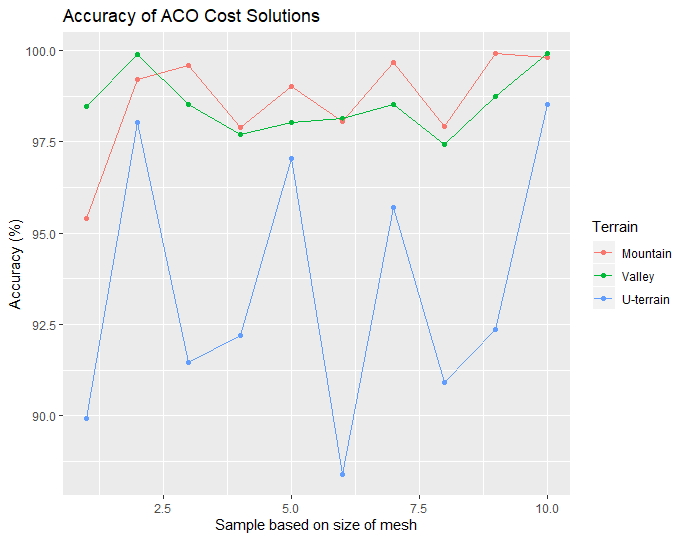
\includegraphics[width=0.7\textwidth]{images/accuracy_example_fig.png}
    \caption{Figure's description.}
     \label{fig:description}
\end{figure}

\chapter{State of the Art}
\label{chap:state_of_art}
[State of the art]

%\chapter{Problem Setting}
%label{chap:problem_setting}
%problem setting

\chapter{Methodology}
\label{chap:methods}

\section{Phases of Problem Solving}


\subsection{Description of the Problem}



\subsection{Analysis of the Problem}



\subsection{Algorithm Design}



\subsection{Implementation}

\subsection{Testing}


\section{Model Proposal}


\section{Experimental Setup}


\chapter{Results and Discussion}
\label{chap:results}
[Your results here]


%\chapter{Discussion}
%\label{chap:results}
%your discussion


\chapter{Conclusions}
\label{chap:conclusions}
[Your conclusions]




%%%%%%% Bibliography %%%%%%%%
\bibliographystyle{bst/IEEEtran} 
\bibliography{bib/IEEEreferences} 
%%%%%%% Bibliography %%%%%%%%    

\appendix  
\clearpage % o \cleardoublepage
\addappheadtotoc 
\appendixpage 

\section{Appendix 1. }
[Your appendix]



\end{document}